%++++++++++++++++++++++++++++++++++++++++
% Don't modify this section unless you know what you're doing!
\documentclass[letterpaper,12pt]{article}
\usepackage{tabularx} % extra features for tabular environment
\usepackage{amsmath}  % improve math presentation
\usepackage{graphicx} % takes care of graphic including machinery
\usepackage[margin=1in,letterpaper]{geometry} % decreases margins
\usepackage{cite} % takes care of citations
\usepackage{todonotes}
\usepackage[final]{hyperref} % adds hyper links inside the generated pdf file
\hypersetup{
	colorlinks=true,       % false: boxed links; true: colored links
	linkcolor=blue,        % color of internal links
	citecolor=blue,        % color of links to bibliography
	filecolor=magenta,     % color of file links
	urlcolor=blue         
}
%++++++++++++++++++++++++++++++++++++++++

\begin{document}

\title{Vowel Recognition}
\author{}
\date{\today}
\maketitle

\section{Introduction}

Speech recognition is a technology that has had a lot of improvement in recent years. While common knowledge indicates that consonants are the most dominant features in recognizing words, sometimes words consist of purely voiced utterances. For instance we can not distinguishing between words like ``man'' and ``moon'' by considering only the consonants. We can see that the proper speech recognition also requires robust recognition of voiced features. In this report, we explore methods to differentiate all the vowels from each other using machine learning methods. Our experiments focus on classifying unambiguously uttered vowels ``a'', ``e'', ``i'', ``o'' and ``u''.

The proper goal of this project is creating a decent vowels classifier. In Section \ref{sec:problem-formulation}, we formalize the vowel recognition problem into a machine learning problem, and furthermore in Section \ref{sec:methods}, we explain our methods of data refinement. 

\section{Problem Formulation}\label{sec:problem-formulation}

The commonly recognized features of a voiced utterance are intensity, pitch and timbre. Out of these features timbre, or the ``fine detail'', is the one that we can use to differentiate between vowels. When pressure is plotted as a function of time, timbre is defined by the shape of a single wavelength. On the frequency side timbre is encoded in the energy distribution. We will use the latter representation of sound waves as our features.

A Fourier transform of a sound wave expresses it as a sum of sine waves. Furthermore, the energy of a sine wave is proportional to the squares of the the amplitude and frequency. In summary, it is as follows: 
\begin{equation}
E\propto A^2\omega^2
\end{equation}
One idea is to use the logarithmic energy distribution of the utterance's Fourier transforms between the frequencies $60$ and $6000$ Hz sampled at $60$ Hz intervals as our sole feature. This one feature can be seen as a composition of $100$ ``smaller'' features. Our labels will be the letters a, e, i, o and u. Since we are working with labeled data, our task falls to the category of supervised learning.

\subsection{Dataset}

We are using the DATASET\_OF\_VOWELS that can be found in Kaggle\cite{dataset} as our base dataset. The base dataset consists of roughly $1600$ labeled utterances from multiple different speakers. The utterances are vowels and are evenly distributed among a, e, i, o and u.

\section{Methods}\label{sec:methods}

\subsection{Dataset parsing}

The base dataset requires heavy processing so that it fits our problem formulation. Here is a brief description of our processing methods: We split the original audio files to suitably sized time windows and take the Fourier transforms of those windows. We use a pitch detector to filter out unvoiced datapoints and pick ten samples from each audio file. The energy distributions of the samples are stored in csv format. For more details, see the bottom part of parser/tasks/parser.cpp in the Github repository \cite{repo}. We obtain Figure \ref{fig:figenergy} when we plot the mean energy distributions of the datapoints. From the medians alone we can determine that our choice of features will be sufficient since the shapes are so different. In the feature space this corresponds to the clusters being far apart from each other.

In the end, we ended up generating two datasets. One contains the energy distributions and the other contains only the amplitude distributions. Both consist of around $16000$ datapoints evenly distributed between the labels. The datasets are further split to training sets and testing sets: $20\%$ of an original set goes to the testing set and the rest goes to the training set. Since our data is evenly balanced among the labels we do not need a large test set. At the same time, a bigger training set reduces the risk of overfitting.

\begin{figure}
    \centering
    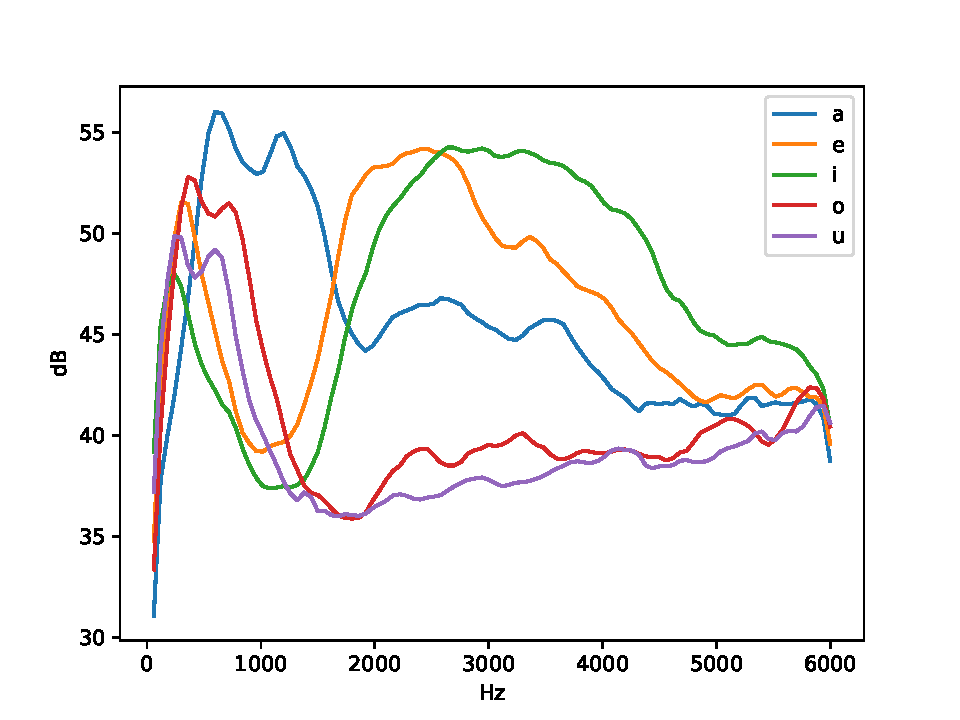
\includegraphics[scale = 0.8]{energy_distribution.pdf}
    \caption{The mean energy distribution of vowels}
    \label{fig:figenergy}
\end{figure}

\subsection{Logistic regression}

Since the clusters' centers of mass are far apart from each other, using logistic regression should produce decent results. Therefore logistic loss is an easy choice of loss function in the training phase. We will use 0/1 loss in the testing phase and visualize the results as a confusion matrix. Based on the visualization of the dataset in Figure \ref{fig:figenergy}, we expect the model to clearly recognize ``a'', ``e'' and ``i'' while ``o'' and ``u'' will get confused more often. This is indeed what happens as we can see from the confusion matrix in the Figure \ref{fig:figconfusion}. The total accuracy of this model turns out to be $85\%$ with the amplitude dataset. This is significantly higher than the result we obtain with the energy dataset, which scored $80\%$ in accuracy.

\begin{figure}
    \centering
    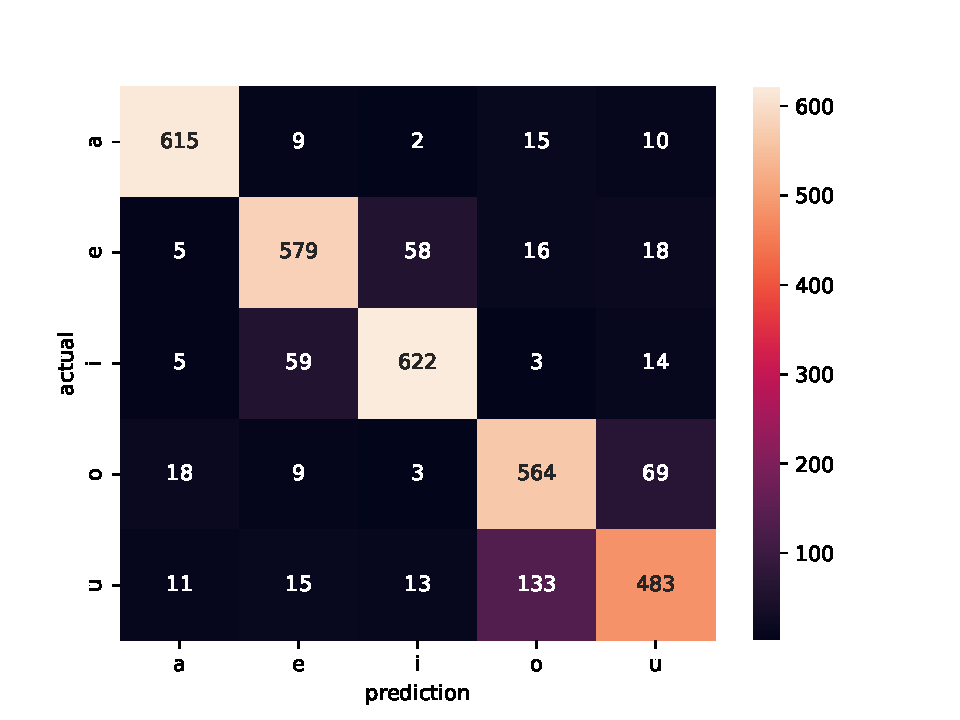
\includegraphics[scale = 0.8]{logistic_confusion.pdf}
    \caption{The confusion matrix obtained with logistic loss}
    \label{fig:figconfusion}
\end{figure}
\begin{thebibliography}{99}
\bibitem{dataset} DATASET\_OF\_VOWELS, available at \\ \href{https://www.kaggle.com/datasets/darubiano57/dataset-of-vowels?resource=download}{https://www.kaggle.com/datasets/darubiano57/dataset-of-vowels?resource=download}.

\bibitem{repo} Github repository, available at \\\href{https://github.com/UnilK/ML-project}{https://github.com/UnilK/ML-project}.
\end{thebibliography}

\end{document}
